\documentclass[a4paper,11pt]{article}
\usepackage{subfiles}
\usepackage{modules/f420}

\title{Geodesics, Shortest Paths, and Non-Isomorphic Nets}
\author{{\scshape Potvin} Nicolas \and {\scshape Zolotov} Boris}
\date{ULB,\quad November 2020}

\begin{document} \maketitle

\section{Introduction}

Given a collection of 2D polygons, a \emph{gluing} or a \emph{net} describes a closed surface by specifying how to glue (a part of) each edge of these polygons onto (a part of) another edge. Alexandrov's uniqueness theorem~\cite{alex} states that any valid gluing that is homeomorphic to a sphere and that does not yield a total facial angle greater than $2\pi$ at any point, corresponds to the surface of a unique convex 3D polyhedron (doubly covered convex polygons are also regarded as polyhedra). Note that the original polygonal pieces might need to be folded to obtain this 3D surface.

Unfortunately, the proof of Alexandrov's theorem is highly non-constructive. The only known approximation algorithm to find the vertices of this polyhedron~\cite{kpd09-approx} has a (pseudopolynomial) running time really large in $n$, where $n$ is the total complexity of the gluing.

There is no known exact algorithm for reconstructing the 3D polyhedron, and in fact the coordinates of the vertices of the polyhedron might not even be expressible as a closed formula~\cite{bannister2014galois}.

Enumerating all possible valid gluings is also not an easy task, as the number of gluings can be exponential even for a single polygon~\cite{DDLO02}. However one valid gluing can be found in polynomial time using dynamic programming~\cite{DO07,lo96-dynprog}. Complete enumerations of gluings and the resulting polyhedra are only known for very specific cases such as the Latin cross~\cite{ddlop99} and a single regular convex polygon~\cite{DO07}.

The special case when the polygons to be glued together are all identical regular $k$-gons, and the gluing is \emph{edge-to-edge} was studied recently for $k \ge 6$~\cite{kl17-hex} and $k=5$~\cite{alz-penta}. The aim of this project is to study the case of $k=4$.

\section{Nicolas' part: implementation of Chen—Han Algorithm}
Chen—Han algorithm is presented in~\cite{chen-han}. It is needed to build knowledge about the gluing. It has to be generalized from the case of the net of a polyhedron to an arbitrary gluing where polygons need not to be faces.\par
The API built to interface Chen \& Han will be the core of this part and serve to demonstrate the algorithm through interactive examples coded in JavaScript. The aim is to propose an educational resource to explain this algorithm in an intuitive and visual manner.\par


\section{Boris' part: enumeration of gluings, isomorphism check}

Estimate of the number of vertices, enumeration of gluings was done in~\cite{kl17-hex,alz-penta}.

\section{Application Programming Interface}
Both parts of the work will be connected through an API. Two main functions have been identified so far:
\begin{itemize}
  \item Given a net, return the number of vertices that are part of the polyhedrons.
  \item Given a net, return a square matrix of dimensions $|V|\times|V|$. This matrix holds the distances between any two pairs of vertices, computed using the Chen \& Han algorithm.
\end{itemize}

The format used to represent a net is an array of $n$ arrays of $k$ oriented line segments. The number $n$ is arbitrary, but the number $k$ is fixed to either $3$ or $4$ to handle respectively the classical situation where triangles are used and the the more specific situation of a net made of squares.

When gluing squares of the same size edge-to-edge, we can forget about the segments and only store the numbers that represent the equivalence class that the edge belongs to. The orientation in which to glue the edges and the net itself can be reconstructed from this data immediately, see Figure~\ref{fig:squaresGlue}.

\begin{figure}[h] \centering
	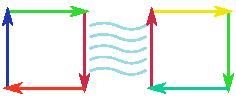
\includegraphics[width=0.35\textwidth]{squares-glue}
	\caption{The information about two edges of squares belonging to the same equivalence class is enough to reconstruct the way they are glued.}
	\label{fig:squaresGlue}
\end{figure}

\subsection{Triangles and squares}
When working on triangles, the Chen \& Han algorithm is unchanged. The issue arising from the use of squares instead is that a geodesic can go through a single square more than once. Since the algorithm does not come back on a previously visited shape, this means that the algorithm needs to be slightly modified.

The idea is to run it longer to allow visiting again previously encountered squares. As proven in~\cite{z-bachthesis}, the number of times a path goes through a single square is at most $7$, which provides an upper bound on the number of steps of the modified algorithm.


\bibliography{boris-bac}{}
\bibliographystyle{plain}

\end{document}
